\chapter{The Standard Model and Physics of the Top Quark}
\label{c:the_standard_model_and_top_physics}

\section{The Standard Model}
\label{s:the_standard_model}

The Standard Model is the name given to the theory developed during the course of the 20th century, which
describes the elementary particles that make up all known, observable matter, and the three fundamental forces
they interact by (electromagnetic, weak and strong forces). The Standard Model does not, however, describe the
gravitational force as it is difficult to model mathematically at a quantum scale.
% The theory is a combination of the theory of the electroweak interaction and the theory of the strong
% interaction
The Standard Model puts forward twelve fermions, with a spin quantum number of $\frac{1}{2}$, as the matter
particles, split into two groups of six quarks and six leptons, all of which are split into three generations.
The six quarks are classified according to their charge and flavour: up, down, charm, strange, top and beauty
quarks. The leptons are in turn classified according to their charge and flavour: electron, muon or tau
leptons, together with their corresponding neutrinos). Neutrinos, although originally thought to be massless,
are now believed to carry mass due to the observation of the oscillation of neutrinos between different
flavours. Table~\ref{tab:standard_model} shows these particles of the Standard Model in their respective
generations in tabular form. All of these particles have a respective antiparticle which has identical quantum
numbers except opposite electric charge.

\begin{table}[hbth]
\centering
\begin{tabular}{lllll}
\hline
Generation & Flavour & Charge / $e$ & Spin & Mass /\MeV \\
\hline
\hline
\multicolumn{5}{c}{\textbf{Leptons}} \\
\hline
\multirow{2}{*}{I} & electron (e) & -1 & $\frac{1}{2}$ & 0.511 \\
 & electron neutrino ($\nu_{e}$) & 0  & $\frac{1}{2}$ & 0 \\
\hline
\multirow{2}{*}{II} & muon ($\mu$) & -1 & $\frac{1}{2}$ & 105.66 \\
 & muon neutrino ($\nu_{\mu}$) & 0 & $\frac{1}{2}$ & 0 \\
\hline
\multirow{2}{*}{III} & tau ($\tau$) & -1 & $\frac{1}{2}$ & 105.66 \\
 & tau neutrino ($\nu_{\tau}$) & 0 & $\frac{1}{2}$ & 0 \\
\hline
\hline
\multicolumn{5}{c}{\textbf{Quarks}} \\
\hline
\multirow{2}{*}{I} & up (u) & $+\frac{2}{3}$ & $\frac{1}{2}$ & $2.3^{+0.7}_{-0.5}$ \\
 & down (d) & $-\frac{1}{3}$ & $\frac{1}{2}$ & $4.8^{0.5}_{-0.3}$ \\
\hline
\multirow{2}{*}{II} & charm (c) & $+\frac{2}{3}$ & $\frac{1}{2}$ & $(1.275^{+0.025}_{-0.025}) \times 10^{3}$ \\
 & strange (s) & $-\frac{1}{3}$ & $\frac{1}{2}$ & $95^{+5}_{-5}$ \\
\hline
\multirow{2}{*}{III} & top/truth (t) & $+\frac{2}{3}$ & $\frac{1}{2}$ & $(173.21\pm{0.51}\pm{0.71}) \times 10^{3}$ \\
 & bottom/beauty (b) & $-\frac{1}{3}$ & $\frac{1}{2}$ & $(4.18^{+0.03}_{-0.03}) \times 10^{3}$ \\
\hline
\hline
\multicolumn{5}{c}{\textbf{Bosons}} \\
\hline
Force & Gauge Boson(s) & Charge / $e$ & Spin & Mass /\GeV \\
\hline
Weak & $\W^{+} / \W^{-} / \Z^{0}$ & +/-/0 & 1 & $80.385\pm0.015 / 91.188\pm0.002$ \\
Electromagnetic & photon ($\gamma$) & 0 & 1 & 0 \\
Strong & gluon (g) & 0 & 1 & 0 \\
Gravitation & graviton & 0 & 1 & 0 \\
- & Higgs (H) & 0 & 0 & $125.7\pm0.4$ \\
\hline
\end{tabular}
\caption{Fundamental fermions, split into their three generations, and bosons of the Standard Model.
Particle properties taken from \cite{Agashe:2014kda}.}
\label{tab:standard_model}
\end{table}



All known, observable matter in the universe is composed of the aforementioned twelve fermions or their
antiparticles. The only particles which are stable are the proton, which is made of two up quarks and a down
quark; the neutron, which is made of one up quark and two down quarks; and the electron. All other particles
are unstable and decay; they are produced only in particle colliders such as the Large Hadron Collider, or in
cosmic radiation. Quarks also carry the charge of the strong force, termed 'colour', of red, green or blue.
The only quark which does not 'hadronise' (form bound colourless states) is the top quark which has a
very short lifetime of $\approx 5 \times 10^{-25}s$ \cite{Agashe:2014kda} due to its large mass.

These fermions interact via the integer spin (spin 1) gauge bosons of the three fundamental forces. Electron,
muon and tau leptons interact via the electromagnetic and weak forces; their neutrinos, since they carry no
electric charge, interact only via the weak force; and the quarks interact via the electromagnetic, weak and
strong forces. Each of the forces are mediated by gauge bosons that are the 'force carriers', and lead to the
formation of hadrons and atoms. The mediator of the strong force is known as the gluon, that of the
electromagnetic force is the photon and those of the weak force are the $\W^{+}$, $\W^{-}$ and $\Z$ bosons.
Table~\ref{tab:standard_model} shows the gauge bosons and their properties.

The range of action of the boson determines the interaction range of the force it carries. Heavier bosons,
like the $\W^{+}$, $\W^{-}$ and $\Z$ bosons, have a short range of action, while massless bosons such as
photons and gluons have a theoretically infinite range. In reality, this is not the case because the gluons
themselves carry the strong colour charge and so interact with each other, reducing their interaction range.
The range of the  fundamental forces is quantified by their coupling strength, denoted $\alpha$. Taking the
strength of the strong force as the baseline, the relative strength of the electromagnetic force is $10^{-2}$,
that of the weak force is $10^{-13}$ and the strength of the gravitational force is $10^{-42}$
~\cite{Griffiths:1987tj}. The electromagnetic coupling strength, also known as the fine-structure constant, is
defined at low energies as $\alpha_{em} = \frac{e^{2}}{4\pi}\approx \frac{1}{137}$. Although the strong force
is the strongest force, it has a limited range of only an estimated $10^{-15}$m, and the weak force has an
estimated range of $10^{-18}$m, while the electromagnetic and gravitational forces have infinite range.

The Higgs boson, whose discovery was announced in July 2012 by the CMS and ATLAS experiments at the LHC, is
the latest component of the Standard Model to be discovered \cite{Chatrchyan:2012xdj, Aad:2012tfa}. The
mechanism of electroweak symmetry breaking through which other particles acquire mass is due to this Higgs
field.

\subsection{Gauge Principle}
\label{ss:gauge_principle}
The underlying mathematical model of the Standard Model is a Quantum Field Theory (QFT) combining special
relativity and quantum mechanics. All interactions in the the SM must conserve the kinematic quantities energy
and momentum. In addition, the electromagnetic and strong forces conserve the dynamical quantities charge,
colour, baryon number, lepton number and quark flavour. The weak force, if mediated by a charged propagator
($W^{\pm}$), can allow the violation of quark flavour, meaning a quark can decay into another flavour quark.

The laws of conservation occur as a result of underlying symmetries in the theories; for instance, energy
conservation stems from time symmetry and angular momentum conservation is a result of rotational symmetry.
In addition to these classical symmetries, a quantum field theory can also possess gauge symmetries. The
principle of gauge invariance refers to field theories in which the Lagrangian, which summarises the dynamics
of the system, is invariant under local transformations (transformations that are a function of, and therefore
different at all space-time points in, a field). The collection of all such transformations, called gauge
transformations, are called the Lie group. If the Lie group is commutative, \ie any order of application of
the symmetry transformations produces the same result, the theory is termed Abelian. Conversely, if the group
is non-commutative, the theory is non-Abelian. Each Lie group has an associated generator, and each generator
has a corresponding vector field, or gauge field, whose purpose is ensuring invariance under local
transformations. The quanta of these fields are the gauge bosons of the Standard Model. Note that the converse
of local transformations are global transformations, in which the transformation takes place instantaneously
at all space-time points.
% However, the speed of any tranformation is limited to c, the speed of light, and so a more realistic local
% transformation is interesting to consider.

Group transformations can be represented as groups of $n \times n$ matrices which possess properties such as
unitarity ($U$) and orthogonality ($O$). A group of matricies with determinant 1 is called 'special' ($S$),
leading to further groups of $SU(N)$ and $SO(N)$. The Standard Model is comprised of electroweak theory
(combining electromagnetism and weak theory) a gauge group of $SU(2) \times U(1)$ and the theory of strong
interactions that has a gauge symmetry of $SU(3)$. The Standard Model is therefore a gauge theory based on the
gauge group $SU(3) \times SU(2) \times U(1)$.

\subsection{Quantum Electrodynamics}
\label{ss:quantum_electrodynamics}

Quantum electrodynamics (QED) is a component theory of the Standard Model that governs the interactions of
electrically charged particles. The simplest electromagnetic process is shown in
Figure~\ref{fig:qed_processes}a, and all real processes are made of some number of these processes combined
together, such as electron-positron annihilation shown in Figure~\ref{fig:qed_processes}b.

\begin{figure}[hbtp]
   \centering
     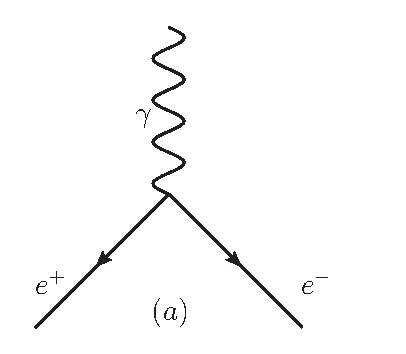
\includegraphics[width=0.3\textwidth]{Chapters/02_Theory/Images/e_e_gamma}\hfill
     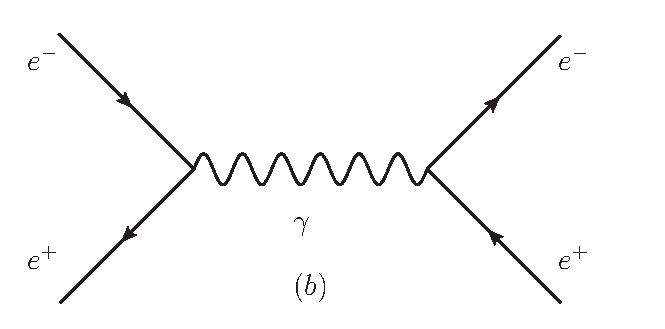
\includegraphics[width=0.5\textwidth]{Chapters/02_Theory/Images/e_e_gamma_e_e}
     \caption{(a) the elementary electromagnetic process of an electron emitting a photon and (b)
     electron-positron annihilation.}
     \label{fig:qed_processes}
\end{figure}


The sum of all possible orders of Feynmann diagrams for a possible interaction is the representation of the
real process. In practice, since at low energies, each vertex contributes a factor of $\alpha$
($=\frac{1}{137}$, the fine structure constant, the coupling constant of the electromagnetic force),
additional Feynmann diagrams with more than a few vertices contribute negligibly to the process and are often
ignored.

The coupling strength of a force can be further explained in terms of vacuum polarisation. This refers to the
phenomenon of electron-positron pairs and photons being spontaneously created and absorbed by an electron.
These virtual particles, which would be represented in Feynmann diagrams as closed loops, shield the original
electron leading to the electron charge being measured at a lower value than its true charge. This measured
value is called the effective, or 'screened', charge. As a result, the coupling strength of the
electromagnetic force decreases as a function of distance.

The mathematical formulation of QED stems from the Dirac equation, which describes the Lagrangian for a
spin-half (Fermionic) field $\psi$.

\begin{equation}
\calL = i (\hbar c) \bar{\psi} \gamma^{mu} \partial_{\mu} \psi - (mc^{2}) \bar{\psi} \psi
\end{equation}

Here, $\hbar$ is the reduced Planck's constant, $\mu$ are the Lorentz indices and $\gamma^{mu}$ are the gamma
(or Dirac) matrices. Under a global transformation of a phase $i \alpha$, 

\begin{equation}
\psi(x) \rightarrow \psi'(x) = e^{i\alpha}\psi(x), \bar{\psi} \rightarrow \bar{\psi}'(x) =
e^{-i\alpha}\bar{\psi}(x)
\end{equation}

this Lagrangian is invariant (\ie under a global transformation of the $U(1)$ group, since this is
equivalent to multiplication of the field $\psi$ by a $1 \times 1$ unitary matrix). However, under a local
gauge transformation by a phase of $i\alpha(x)$, the symmetry is no longer true since the partial derivative

\begin{equation}
\partial_{\mu}(e^{i\alpha(x)}\psi) = i(\partial_{\mu}\alpha(x))e^{i\alpha(x)}\psi +
e^{i\alpha(x))}\partial_{\mu}\psi ,
\end{equation}

meaning the Lagrangian is not invariant:

\begin{equation}
\calL \rightarrow \calL - \bar{\psi}(x)\gamma^{\mu}\psi(x)[\partial_{\mu}\alpha(x)].
\end{equation}

Local symmetry can be maintained in this case if a new gauge field, $A_\mu$, is introduced to the Lagrangian
by means of a covariant derivative $D_\mu$:

\begin{equation}
D_{\mu} = \partial_{\mu} + ieA_{\mu}.
\end{equation}

Under the local transformation, $A_{mu}$ tranforms as

\begin{equation}
A_{\mu} \rightarrow A_{\mu}' = A_{\mu} - \frac{1}{e}\partial_{\mu}\alpha(x).
\end{equation}

If the partial derivatives in the Dirac equation are now replaced with the covariant derivatives, the
invariant Lagrangian is obtained:

\begin{equation}
\calL = i (\hbar c) \bar{\psi} \gamma^{mu} \partial_{\mu} \psi - e \bar{\psi} \gamma^{\mu} \psi A_{\mu} -
(mc^{2}) \bar{\psi} \psi - \frac{1}{4}F^{\mu\nu}F_{\mu\nu}.
\end{equation}

In this way, the principle of local gauge invariance under the $U(1)$ group is used to obtain the final
Lagrangian, that of quantum electrodynamics. The physical interpretation of the gauge field $A_{\mu}$ is the
photon, which couples to charged particles (electrons and positrons) with a coupling strength proportional to
the charge. The term $\frac{1}{4}F_{\mu\nu}$ is an additional term to account for the kinetic energy of the
free particle of the new gauge field, \ie the photon; and there is no term giving the photon mass.

% \begin{equation}
% F_{\mu\nu} = \partial_{\mu}A_{\nu} - \partial_{\nu}A_{\mu}.
% \end{equation}

In this way, the principle of local gauge invariance under the $U(1)$ group is used to 
introduce additional
fields to a Lagrangian in order to make it covariant with respect to a group  $U(1)$ local gauge invariance

\subsection{Electroweak Theory}
\label{ss:electroweak_theory}

The unification of the electromagnetic and weak forces in the 1960s provided a more complete theory of
fundamental particles. This unification takes the form of an $SU(2) \times U(1)$ gauge group correlating the
electromagnetic and weak forces, and can be constructed in a similar way to the QED formalism in
Section~\ref{ss:quantum_chromodynamics}. 

First, it is necessary to define isospin, $I$ an abstract fundamental property of fundamental particles that
is conserved in weak interactions. Similarly, weak hypercharge, $Y$ is also a quantum property, defined as
$Y_{W} = 2(Q-I_{3})$, where $Q$ represents the charge of the particle and $I_{3}$ is the third component of
isospin. $I_{3}$ takes a value of $\frac{1}{2}$ for up, charm and top quarks and for neutrinos; and
$-\frac{1}{2}$ for down, strange, beauty and other leptons other than neutrinos.

It has been shown empirically that the weak interaction exhibits violation of parity ($P$) and interacts
only with left-handed particles via the charged gauge bosons ($W^{\pm}$). Hence, the fields representing
fermions are split into left handed and right handed components by defining a left handed doublet
containing the left handed electron and left handed neutrino, and a right handed singlet containing the right
handed electron:
\begin{equation}
\chi_{L} = \left( \begin{array}{c} \nu_{e} \\ e \end{array}\right)_{L}, e_{R}
\end{equation}
Here, the left handed doublet has $I=\frac{1}{2}$, and the right handed lepton has $I = 0$. Similar doublets
can be constructed for the other generations of leptons ($\mu$ and $\tau$) and quarks in their pairs of three
generations ($ud$, $cs$ and $tb$). Right handed neutrinos, which would have $I=0$ and $Y=0$, do not exist in
the Standard Model. %as they would not interact with any of the force mediators.

Four additional massless fields and their associated currents are introduced in order to impose invariance:
$W_{\mu}^{1}$, $W_{mu}^{2}$, $W_{mu}^{3}$ and $B_{\mu}$. The $W_{\mu}$ fields form a triplet that transforms
according to the $SU(2)$ group, and undergoes interactions with the third isospin component $I_{3}$. The
$B_{\mu}$ field similarly transforms by the unitary group $U(1)$, and interacts with the weak hypercharge $Y$.
These additional fields lead to the construction of three weak isospin currents and a weak hypercharge
current.

Requiring local gauge invariance under a the $SU(2) \times U(1)$ group, the covariant derivative is
\begin{equation}
D_{\mu} = \partial_{\mu} + \frac{i}{2} g_{W} \vec{\tau} \cdot \vec{W}_{\mu} + ig' \frac{Y}{2}B_{\mu}.
\end{equation}
The vectors $W_{\mu}^{1}$, $W_{\mu}^{2}$, $W_{\mu}^{3}$ have coupling strengths of $g_{W}$ to the three
isospin currents and $B_{\mu}$ couples to the hypercharge current with a strength of $g'$. These four bosons
relate to the quanta of the new fields, \ie the gauge bosons $W^{\pm}$, $Z^{0}$ and $\gamma$. In actual fact,
the $W^{\pm}$ bosons are linear superpositions of the $W_{\mu}^{1}$ and $W_{\mu}^{2}$ states, while the
neutral states $W_{\mu}^{3}$ and $B_{\mu}$ undergo a mixing related by the weak mixing angle, $\theta_{W}$, to
give the neutral $Z^{0}$ and $\gamma$ bosons. The coupling constants of the electromagnetic and weak forces
are related by the weak mixing angle, by $tan \theta_{W} = \frac{g'}{g_{W}}$.

It has been experimentally observed that both \W bosons and the \Z boson have mass. Indeed, the
strength of the electromagnetic force is of the same order as the weak force, but as a result of the weak
gauge bosons having mass, the weak force appears weaker and has a shorter range. However, the local gauge
invariance would be broken if terms are now included to give the bosons mass. The theory of spontaneous
breaking of the symmetry underlying the $SU(2) \times U(1)$ group addresses this problem, as explained in
Section~\ref{ss:spontaneous_symmetry_breaking}.

The weak force has been shown to change the flavour of quarks in an interaction, meaning flavour conservation
is broken \cite{}. As stated, the quarks, like leptons, come in the form of left handed doublets within each
generation,
\begin{equation}
\left(\begin{array}{c} u_{L} \\ d'_{L} \end{array}\right) , \left(\begin{array}{c} c_{L} \\ 
s'_{L} \end{array}\right) , \left(\begin{array}{c} t_{L} \\ b'_{L} \end{array}\right)
\end{equation}
with isospin $\frac{1}{2}$. Note that the lower quarks of the doublets are denoted with primes as they
indicate a rotated state of the quark, called Cabibbo-rotated states, which are superpositions of the physical quarks.
This means that in, for example, the decay of a down quark to an up quark via emittance of a $\W^{-}$, the
down quark to which the $\W^{-}$ couples is actually a superposition of 'down type' quarks, \ie down, charm and
beauty quarks. The Cabbibo-Kobayashi-Maskawa matrix (CKM), relates the weak interaction mixed states to the
physical quark states. This is the degree of quark mixing between the different generations, and results in
the measured values below of $\abs{V_{12}}$ for the probability of a transition from quark 1 to quark
2 in a weak interaction~\cite{Agashe:2014kda}. In reference to top physics, the \abs{V_{tb}} value of almost 1
means that the top quark almost always decays to a \W boson and a \bquark.

\begin{equation}
\begin{pmatrix}
V_{\cPqu\cPqd} & V_{\cPqu\cPqs} & V_{\cPqu\cPqb} \\
V_{\cPqc\cPqd} & V_{\cPqc\cPqs} & V_{\cPqc\cPqs} \\
V_{\cPqt\cPqd} & V_{\cPqt\cPqs} & V_{\cPqt\cPqb} 
\end{pmatrix}
=
\begin{pmatrix}
0.974 & 0.225 & 0.004 \\
0.225 & 0.973 & 0.041 \\
0.009 & 0.041 & 0.999
\end{pmatrix}
\end{equation}

\subsection{Quantum Chromodynamics}
\label{ss:quantum_chromodynamics}

In the theory of quantum chromodynamics (QCD), the charge of the strong force is colour, and the force is
independent of other particle properties such as charge and flavour. Empirical data has led to the conclusion
that there are three colour charges: red, green and blue \cite{Griffiths:1987tj}. While the colour of a quark
can be changed in a strong interaction, colour conservation is a requirement of strong processes (just as
charge conservation in QED). The mediators of the strong force, gluons, carry a positive and a negative colour
charge themselves, and so can interact directly with other gluons. The coupling constant of the strong force
is a 'running' coupling constant, meaning that it varies depending on the distance between the particles
undergoing the interaction. At small distances of the order of the size of the proton (\~0.1~fm),
$\alpha_{S}$ is small and becomes larger as distance increases, leading to quarks and gluons being essentially
free particles and interacting weakly with each other when confined within a hadron, a phenomenon termed
asymptotic freedom.

The previously mentioned colourless bound quark states are called hadrons. The process in which free gluons
and quarks form bound colourless states is called hadronisation and manifests as a cone of particles, termed
jets. Hadrons are divided into two types: mesons are composed of a quark and an antiquark with the quark
carrying a colour charge and the antiquark carrying the respective anticolour; baryons are composed of three
quarks or three antiquarks. Recently, the LHCb experiment at CERN published first results of the observation
of a pentaquark state ~\cite{Aaij:2015tga} TODO:WORTH MENTIONING? %TODO:WORTH MENTIONING?

The proton, a baryon, consists of two \uquarks, one \dquark and gluons binding the qquarks together. However,
the structure of the proton becomes more complicated, consisting of more particles, as the momentum of the
probing particle increases. The aforementioned three-quark-structure of the proton is evident at low momenta,
while at higher momenta, virtual pairs of quarks, antiquarks and gluons are visible. These virtual quarks and
gluons are termed sea-quarks and make up most of the mass of the proton. In any proton, its constituent
particles each carry some fraction, $x$, of the overall proton momentum. %TODO: At small x (momentum fraction)

The quantum field theory of QCD is determined to have an underlying symmetry of the group $SU(3)$, based on
the fact that there are three colour charges. Imposing local gauge invariance, the Lagrangian contains eight
generators of the $SU(3)$ group. These generators lead to eight gauge fields, whose physical interpretation
are the eight massless gluons that mediate the strong force. Therefore, although in principle there could be
nine gluons, since there are three colours and gluons carry a positive aqnd a negative colour charge, the
$SU(3)$ symmetry leads to a colour octet and a colour singlet. TODO: COULD STATE THEM HERE BUT DON'T THINK
IT'S NECESSARY. % TODO: COULD STATE THEM HERE
%, as shown below:

%\begin{equation}
%\left \{
%(r\bar{b} + b \bar{r})/
%\right \}
%\end{equation}

Any particle that occurs in nature must be a colour singlet, and so the gluons in the colour octet are never
seen in nature. However, although the final gluon is a colour singlet, it has not been observed and is
thought not to exist. If it did exist, it would result in a long range strong force, but it is known that the
strong force has a short range of action.

\subsection{Spontaneous Symmetry Breaking}
\label{ss:spontaneous_symmetry_breaking}

The spontaneous breaking of the electroweak $SU(2)$ symmetry mentioned in Section~\ref{ss:electroweak_theory},
also known as the Higgs mechanism was put forward in the 1960s~\cite{Higgs:1964pj}. This theory was put forward as
a mechanism by which the $\W^{\pm}$ and \Z gauge bosons could acquire mass, since the Lagrangian of the
electroweak interaction contains no mass term for these particles, and their inclusion would violate local
gauge invariance.

The method by which this symmetry is spontaenously broken begins with the inclusion of two new complex scalar
'Higgs' fields (so in total there are four components to these two complex fields). The introduction of these
fields results in an additional scalar potential energy term in the Lagrangian, $V(\Phi)$, where $\Phi$
represents the newly introduced complex scalar fields. %in the form of a doublet.
The potential $V(\Phi)$ is defined as
\begin{equation}
V(\Phi) = -\mu^{2} \Phi^\dagger \Phi + \lambda^{2} (\Phi^\dagger \Phi)^{2}
\end{equation}
%TODO:(WHAT ARE MU AND LAMBDA?)
Imposing the requirement of $\mu^{2}$ and $\lambda$ both being greater than 0 (WHY?), gives a potential of the
geometry shown in Figure~\ref{fig:higgs_potential}. The minimum of this potential is clearly not at
$\Phi=0$, rather, the minimum has a circular form given by the formula $\Phi^\dagger \Phi =
\frac{\mu^{2}}{2\lambda} = \frac{v^{2}}{2}$, where $v = \frac{\abs{\mu}}{\sqrt\lambda}$, the 'vacuum
expectation value' of the Higgs. Since the minimum, \ie the vacuum, is at a location other than $\Phi = 0$,
The new field is said to have a non-zero vacuum expectation value, and the $SU(2) \times U(1)$ symmetry is
spontaneously broken. The observed Higgs boson is created as a result of perturbations in the potential about
this minimum, which removes three of the four $\Phi$ components, with the remaining field being the scalar
Higgs field. %TODO: (WHAT DOES EXPANDING AROUND THE CHOSEN MINIMUM MEAN?)
In addition to this new particle, introducing the new fields also results in the fields associated with the
$\W^{\pm}$ and $\Z^{0}$ bosons in the Lagrangian acquiring mass.
%One of these new fields, $\eta$ and $\xi$. One of these, known as the Goldsone boson, is eaten by the other
%thereby acquiring mass. It is this field that is known as the Higgs field.

\begin{figure}[hbtp]
   \centering
     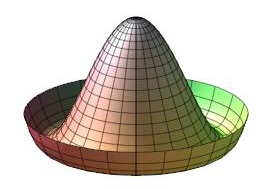
\includegraphics[width=0.5\textwidth]{Chapters/02_Theory/Images/higgspot}\hfill
     \caption{The Higgs field potential $V(\Phi)$~\cite{Moss:2015fma}.}
     \label{fig:higgs_potential}
\end{figure}

Terms known as Yukawa coupling terms can be introduced to specify the interactions of $\Phi$ with the fermion
fields. It is this coupling of the Higgs field to any massive particle that gives them a proportional mass.
The top quark, being the heaviest known particle at ~173\GeV, has a Yukawa coupling to the Higgs close to 1.
%TODO: IMPORTANT BECAUSE?

Results published at the discovery of the Higgs boson are shown in Figure~\ref{fig:higgs_results} in the
Higgs$\rightarrow\gamma\gamma$ and Higgs$\rightarrow\Z\Z$ channels. These plots of the invariant masses of the
$\gamma\gamma$ and $\Z\Z$ combinations show a clear excess of events around 125\GeV. The latest results from
CMS and ATLAS state a Higgs mass of $125.09\pm0.21\pm0.11\GeV$ \cite{Aad:2015zhl}, where the first uncertainty is
statistical and the second is systematic. Since the announcement of the discovery of the Higgs boson in 2012,
studies have continued to determine its quantum properties. Thus far, results show it to be in agreement with
predictions from the Standard Model.

\begin{figure}[hbtp]
   \centering
     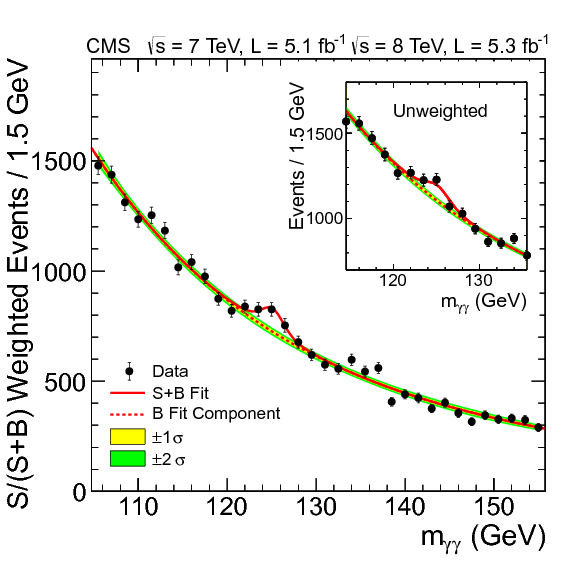
\includegraphics[width=0.5\textwidth]{Chapters/02_Theory/Images/sbweightedmassunweightedinset1_5GeV}\hfill
     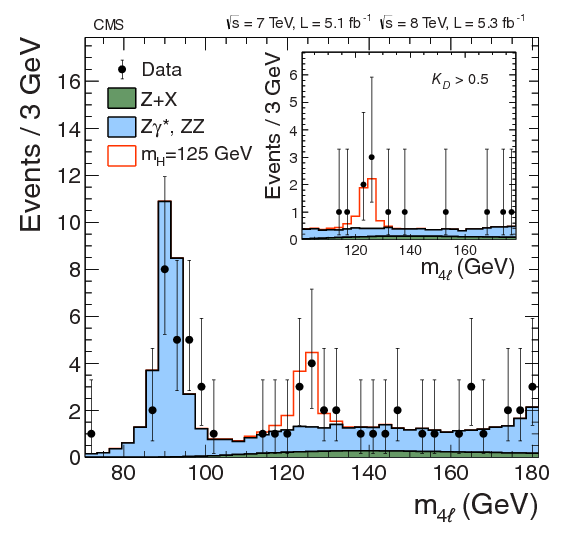
\includegraphics[width=0.5\textwidth]{Chapters/02_Theory/Images/H4l_mass_v3}\hfill
     \caption{Invariant mass in $H\rightarrow\gamma\gamma$ (left) and $H\rightarrow\Z\Z$ (right) channels
     ~\cite{Chatrchyan:2012xdj}.}
     \label{fig:higgs_results}
\end{figure}

\section{Incompleteness of, and physics beyond, the SM}
\label{s:Incompleteness_of_and_physics_beyond_the_SM}
The Standard Model has proven to be an extremely successful theory thus far. However, its inability to
describe many phenomena in the universe lead to it being considered currently incomplete. Indeed, a 'Grand
Unified Theory' combining the electromagnetic, weak and strong interactions is considered to be the ultimate
aim, with all of these forces being different physical manifestations of one single force.

There are many free parameters in the Standard Model and the very reason why it takes the form it has, with
four fundamental forces, six quarks and six leptons, each divided into three generations, is not explained.
The gravitational force is also conspicuous by its absence from the SM. The imbalance between matter and
anti-matter in the universe, despite the generally accepted view that both were created in equal quantities in
the Big Bang, is also not explained by the SM. Although the evident matter-antimatter asymmetry in the
unvierse could be partially explained by the observed charge-parity (CP) symmetry violation in weak
interactions~\cite{Christenson:1964fg}, this is not sufficient to account for the observed excess.

Neither does the SM provide a theoretical explanation for neutrino mass. Originally thought to be massless,
neutrinos are now thought to have mass, albeit extremely small, based on observations of neutrino oscillations
between different flavours~\cite{Kajita:1998bw,Fukuda:1998mi}.

The hierarchy problem, in terms of the Higgs boson, is the name given to the fact that the Higgs mass is so
much smaller than the predicted value of the order of the Planck scale ($1.22\times10^{19}\GeV$). The observed
mass is the sum of the bare particle mass and any corrections from high order processes. This disagreement
suggests that there occurs some 'fine tuning' of the bare Higgs mass to lead to the measured mass of
approximately 125\GeV.

Supersymmetry (SUSY) is one potential solution to hierarchy problem. This theory proposes a symmetry
between fermions (spin $\frac{1}{2}$) and bosons (spin 1). Each particle has an associated 'superpartner' with
identical quantum properties with the exception of spin, which differs by $\frac{1}{2}$, so that all
Standard Model fermions have a boson superpartner, and all Standard Model bosons have a fermion superpartner.
These super particles, or sparticles, are thought to have higher masses than their Standard Model counterparts
since they have not been discovered yet. If this is the case, supersymmetry would be a broken symmetry. In
many supersymmetry theories, the lightest SUSY particle (LSP) is stable and is a potential candidate to be
a dark matter particle.

Dark matter and dark energy are thought to constitute about 27\% dark matter, 68\% dark energy and 5\%
ordinary matter (Figure~\ref{fig:universe_composition}) ~\cite{Ade:2013sjv}. The origins and nature of the
dark energy and dark matter are currently unknown and they are as yet unobserved, but their existence has been
inferred from their gravitational effects on galactic masses composed of stars, gases and dust. The relatively
large amounts of dark matter and dark energy hypothesised suggests that they are made up of weakly interacting
massive particles.

\begin{figure}[hbtp]
   \centering
     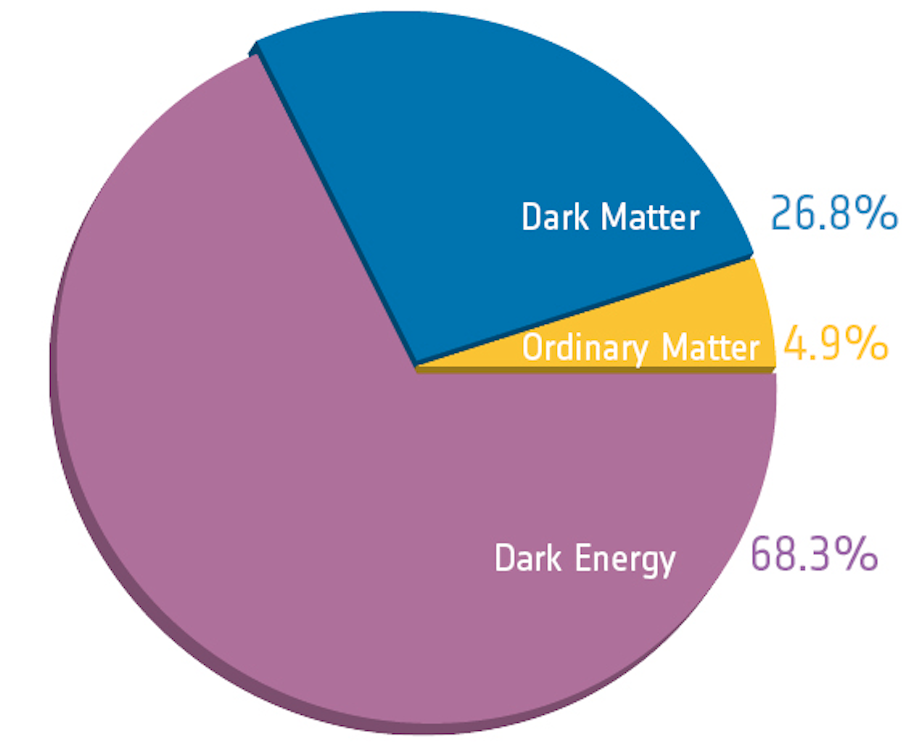
\includegraphics[width=0.5\textwidth]{Chapters/02_Theory/Images/planck_cosmic_pie}\hfill
     \caption{The composition of the universe showing the amounts of dark matter, dark energy and ordinary
     matter based on latest results from Planck/ESA~\cite{Ade:2013sjv}}
     \label{fig:universe_composition}
\end{figure}


\section{Top Physics at the LHC}
\label{s:top_physics_at_the_lhc}
The top quark was discovered by the CDF and D{\O} collaborations in 1995 \cite{Abe:1995hr, Abachi:1995iq} and
is still one of the less well studied fundamental particles in the Standard Model. The top quark is the
heaviest fermion with its mass currently placed at $173.29 \pm 0.23 (stat.) \pm 0.92
(syst.)\mathrm{~GeV/c^{2}}$ \cite{top_mass}. Since the lifetime of the top quark is very short, approximately
$5 \times 10^{25}\mathrm{~s}$ \cite{Agashe:2014kda}, it is the only one of the quarks to decay before it
hadronises, meaning that the bare quark properties can be investigated. These unique properties of the top
quark within the Standard Model mean it is an interesting focus of study.

\subsection{Top Quark Production and Decay}
\label{ss:top_quark_production_and_decay}
Top quarks can be produced either in top-antitop (\ttbar) production through the strong interaction or single
top (\tquark) production through the electroweak mechanism. During Run 1 of data taking at the LHC produced
millions of top quark pair events with gluon-gluon fusion or quark-antiquark annihilation being the primary
production mechanisms, as shown in Figure~\ref{fig:ttbar_production}. Gluon-gluon fusion dominates at the LHC
since protons are collided with protons, meaning antiquarks are only available from sea quarks in the proton.
In addition, at low momentum fractions, $x$, the gluon density in the proton is large compared to the sea
quarks, and increases at a higher rate than that of the sea quarks. TODO: COULD INSERT PLOT OF PROTON
PDFs IF NEEDED %TODO: COULD INSERT PLOT OF PROTON PDFs IF NECESSARY.

\begin{figure}[hbtp]
   \centering
     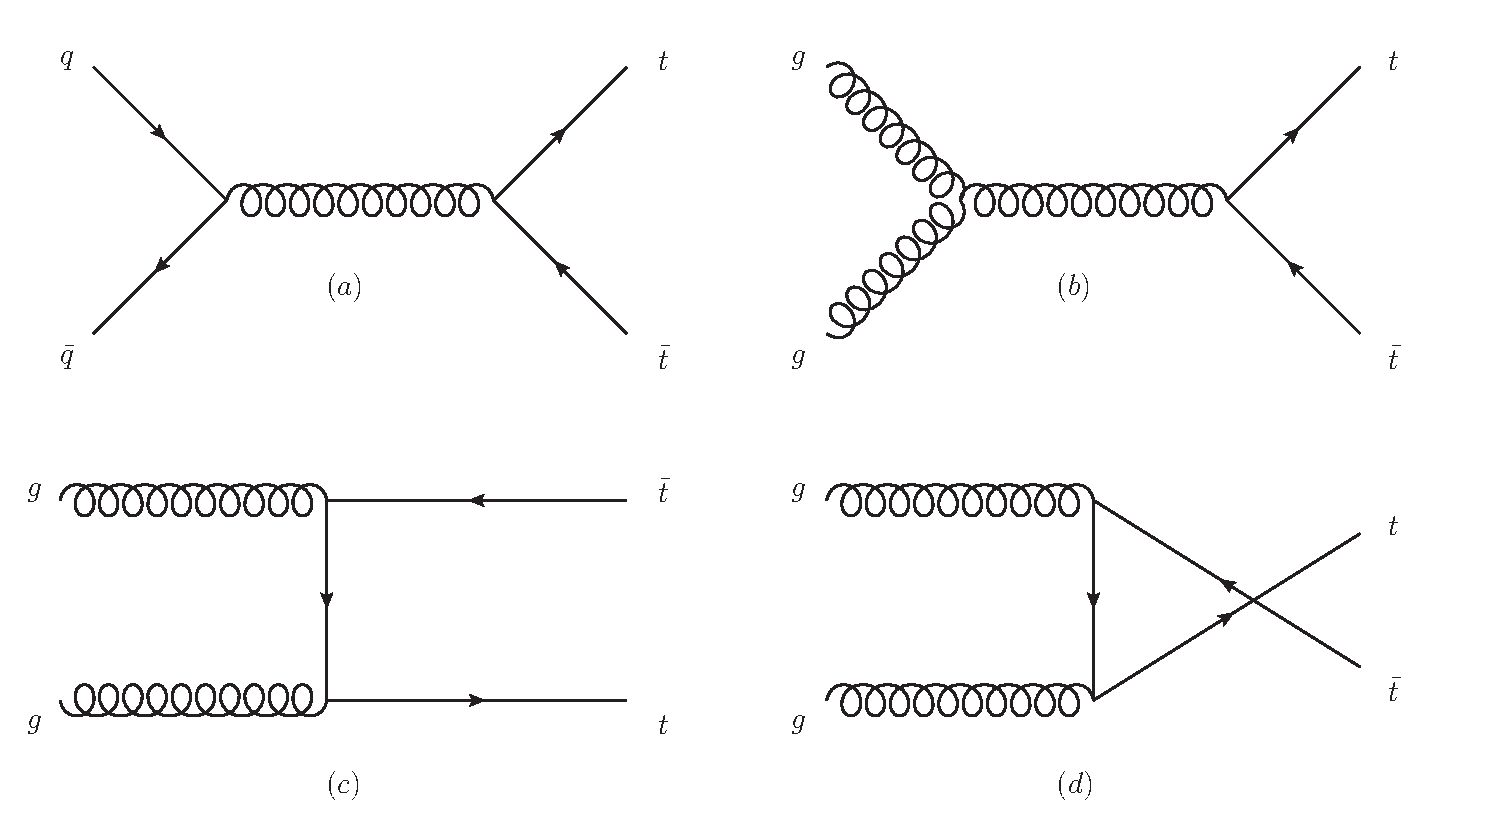
\includegraphics[width=0.9\textwidth]{Chapters/02_Theory/Images/ttbar_production}\hfill \caption{Feynman
     diagrams of leading order \ttbar production processes. (a) depicts quark-antiquark annihilation, and (b,
     (c) and (d) depict gluon-gluon fusion in the s, t and u channels respectively.)}
     \label{fig:ttbar_production}
\end{figure}

At $\sqrt{s}=7\TeV$, gluon-gluon fusion accounts for approximately 80\% of the total \tquark production cross
section, increasing to approximately 90\% at $\sqrt{s}=14\TeV$ \cite{Agashe:2014kda}.
% A \ttbar production cross section of has been measured at $\sqrt{s}=7\TeV$ and at $\sqrt{s}=8\TeV$.

\begin{figure}[hbtp]
   \centering
     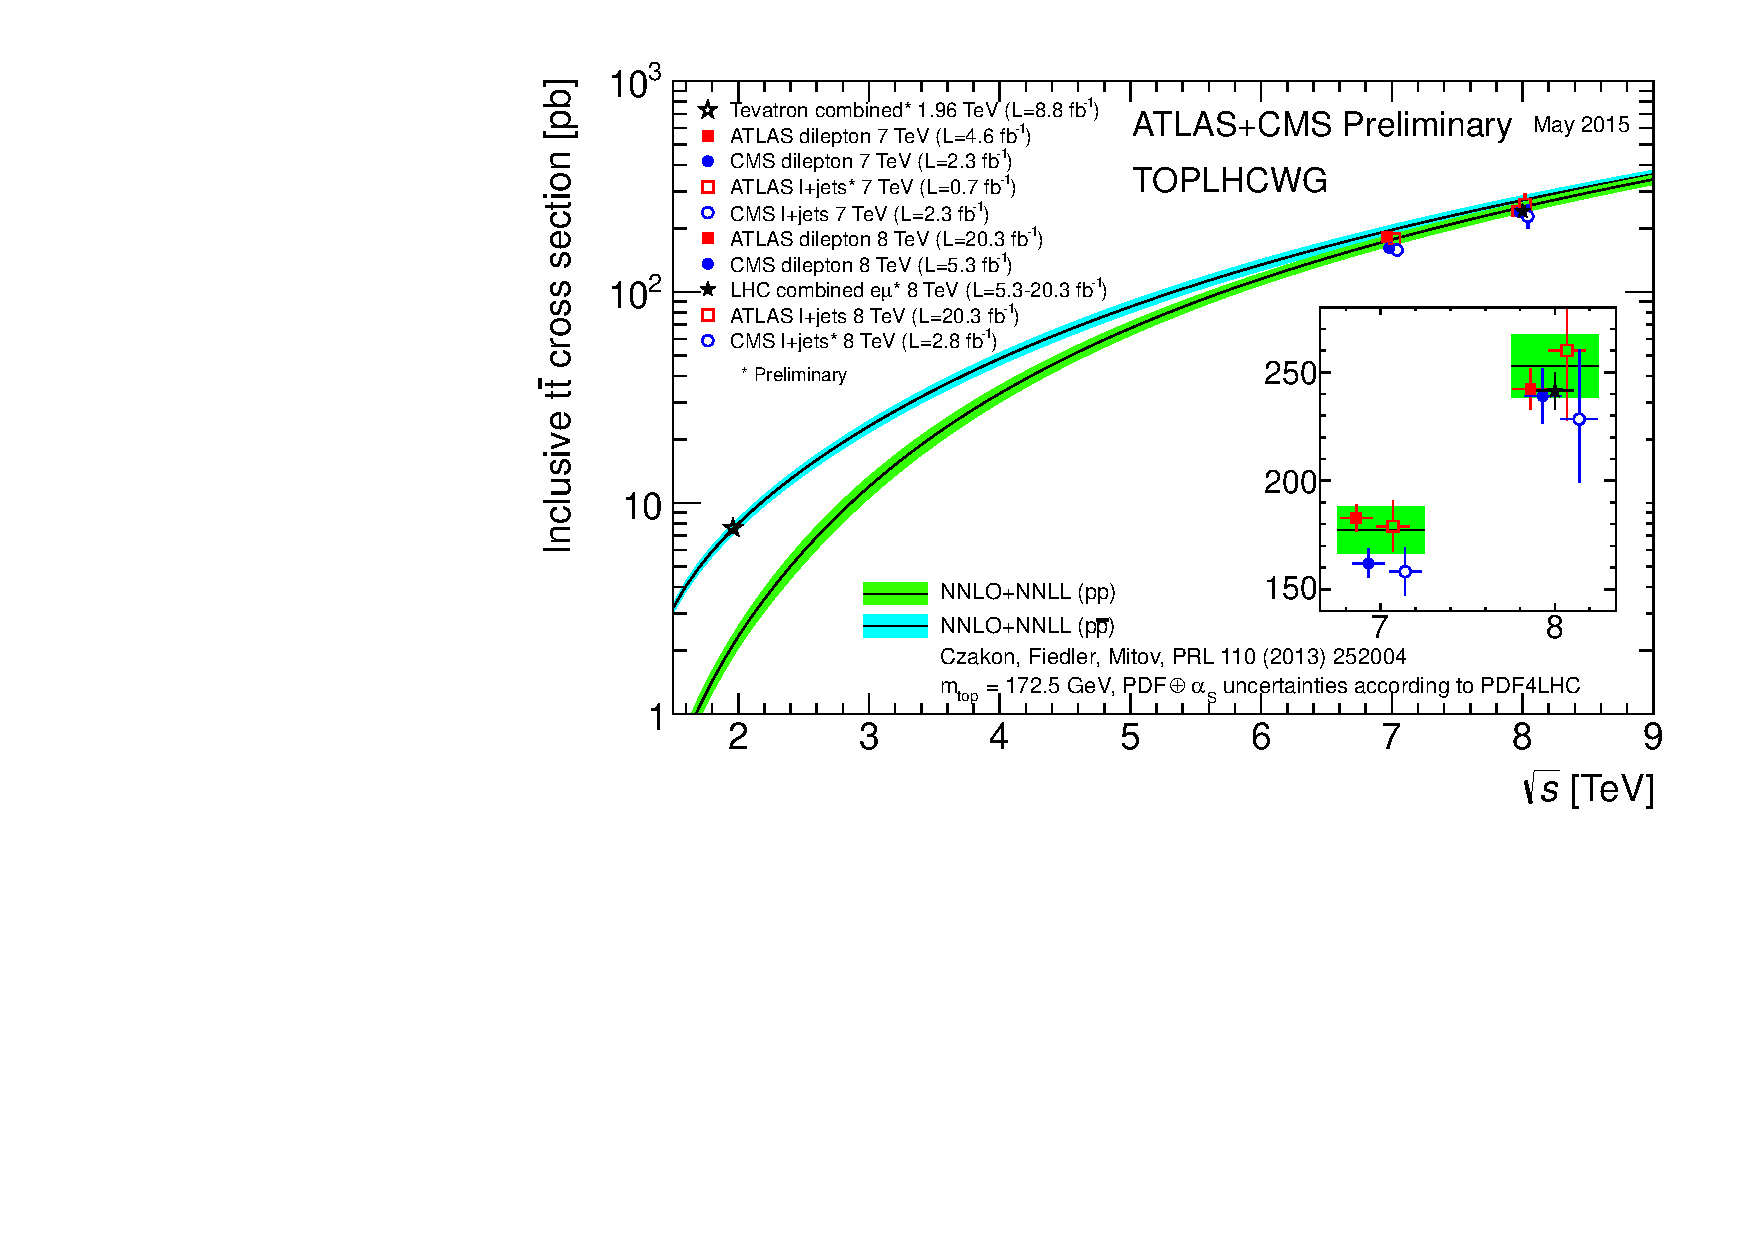
\includegraphics[width=0.5\textwidth]{Chapters/02_Theory/Images/toplhcwg_ttxsec_sqrts_may2015}\hfill
     \caption{\ttbar production cross sections at 1.96\TeV at CDF and D{\O} at the TeVatron and at 7\TeV and
     8\TeV at CMS and ATLAS at the LHC. HOW REFERENCE IMAGE FROM
     https://twiki.cern.ch/twiki/bin/view/LHCPhysics/TopLHCWGSummaryPlots?}
     \label{fig:ttbar_cross_sections}
\end{figure}

Top quarks decay almost 100\% of the time to a W-boson and a b flavour jet. The W-boson then decays either
hadronically (into two jets) or leptonically (lepton + neutrino). Top pair events are characterised by the
decay of the W-bosons:
\begin{itemize}
  \item Leptonic: $\ttbar \rightarrow \W^{+} \cPqb \W^{-} \cPaqb \rightarrow l \nu_{l}\cPqb
  l' \bar{\nu_{l'}} \cPaqb$.
  Both W-bosons decay to a lepton and a neutrino. The event would consist of 2 jets, 2 leptons and 2 neutrinos (which would show
  up as \met in the event). (10.5\%)
  \item Hadronic: $\ttbar \rightarrow \W^{+} \cPqb \W^{-} \cPaqb \rightarrow \cPq \cPaq \cPqb \cPq \cPaq
  \cPaqb$. Both W-bosons decay to two jets. The event would consist of 6 jets. (45.7\%)
  \item Semi-Leptonic: $\ttbar \rightarrow \W^{+} \cPqb \W^{-} \cPaqb \rightarrow \cPq \cPaq \cPqb l \nu_{l}
  \cPaqb$. One \W-boson decays to a lepton and a neutrino, the other decays to two jets. The event would
  consist of 4 jets, 1 lepton and 1 neutrino. This decay is shown in Figure~\ref{fig:semileptonic_decay}.
  (43.8\%)
\end{itemize}

\begin{figure}[hbtp]
   \centering
     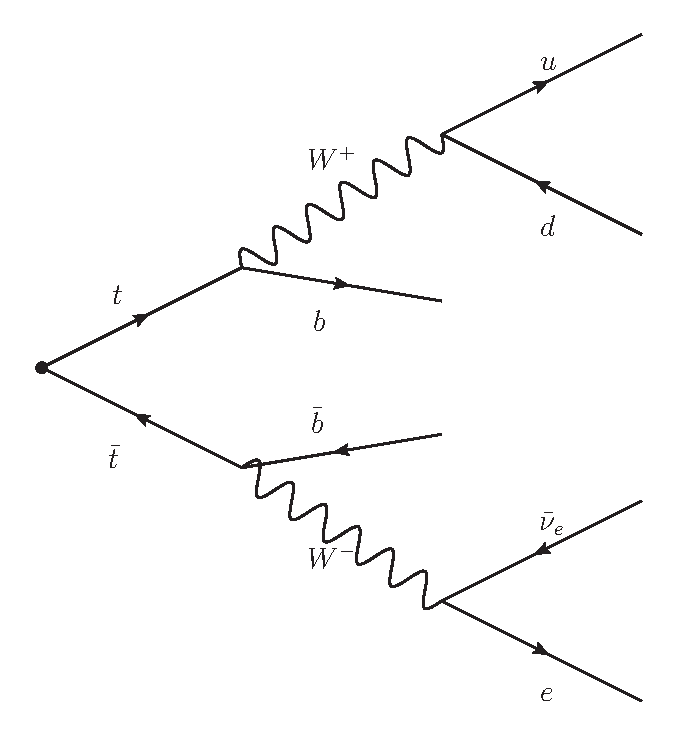
\includegraphics[width=0.5\textwidth]{Chapters/02_Theory/Images/semileptonic_decay}\hfill
     \caption{Feynman diagram of the electron+jets semi-leptonic \ttbar decay channel}
     \label{fig:semileptonic_decay}
\end{figure}

The branching ratios for each decay mode are quoted in brackets \cite{Agashe:2014kda}, and are represented
graphically in Figure~\ref{fig:ttbar_branching_ratios}. The numbers of jets in the final state of each channel
could be higher than the numbers quoted above as a result of higher order processes such as initial state
radiation (radiation from the gluons before the \ttbar production) or final state radiation. The hadronic
decay channel, with multiple jets and no leptons in the final state, is difficult to distinguish from the QCD
multijet, W+jets and Z+jets backgrounds. Conversely, the leptonic channel has a very clean signature with two
leptons, however the low branching ratio would limit the available statistics. The semi-leptonic channel, with
one lepton and four jets provides a good balance between statistics and event identification. The lepton can
be any of an electron, muon or $\tau$, but $\tau$s are not included in semi-leptonic \tquark analyses in
general as they are difficult to identify (see Section~\ref{ss:experimental_uncertainties}).

\begin{figure}[hbtp]
   \centering
     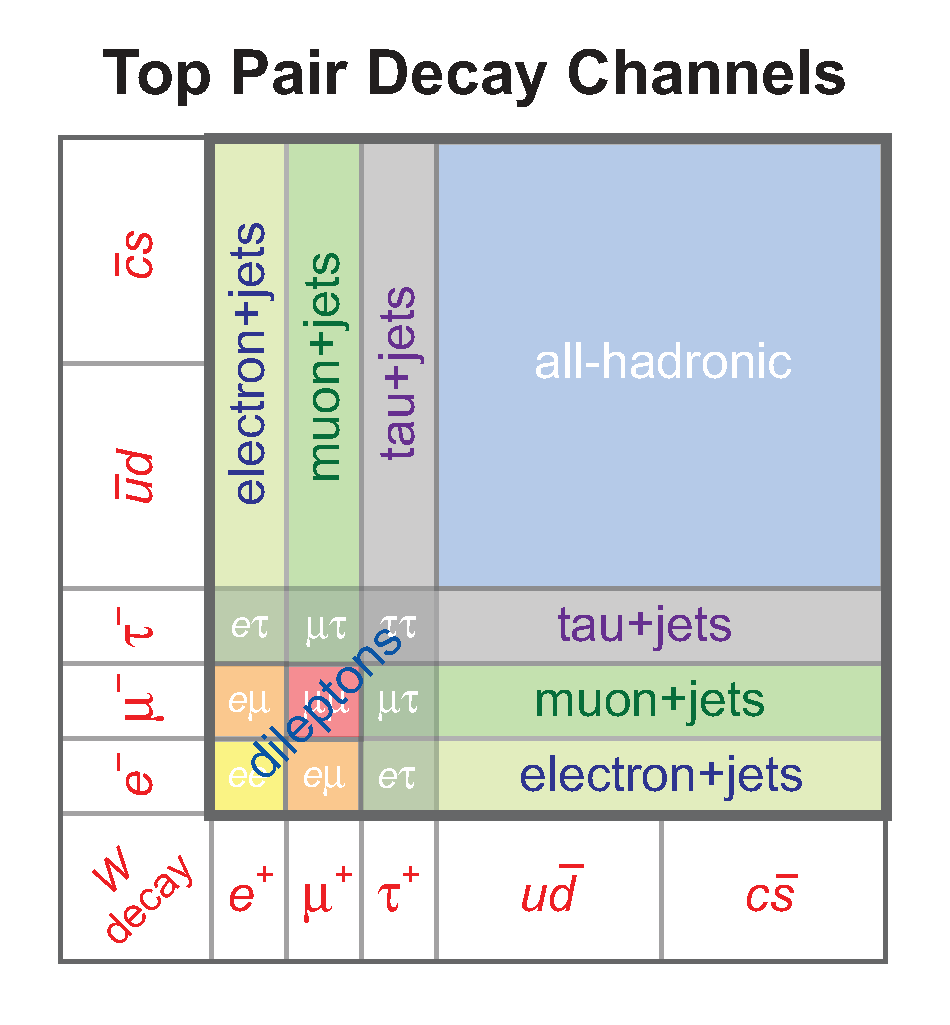
\includegraphics[width=0.5\textwidth]{Chapters/02_Theory/Images/top_pair_decay_channels.eps}\hfill
     \caption{Relative branching ratios of the \ttbar system}
     \label{fig:ttbar_branching_ratios}
\end{figure}

The signal event for this analysis is the semi-leptonic channel of the \ttbar decay, also referred to as
the lepton+jets channel, where the lepton is either an electron or a muon. These channels have a branching
ratio of apprimxately 14.2~\% and 14.4~\% respectively \cite{Agashe:2014kda}.

\subsection{Single Top background}
\label{ss:single_top}
Single top production is one of the backgrounds considered in this analysis, and can occur via the electroweak
interaction in one of three channels: s-channel or t-channel which involve the exchange of a virtual \W boson,
or tW-channel which involves the associated production of a \W boson and a top quark. Although semi-leptonic
\ttbar decays have more jets in the final state than these single top production modes, initial state
radiation and final state radiation, where low energy gluons and quarks are produced before and after the
interaction that produces the single \t quark, can increase the numbers of jets in single top events. This can
lead to such events having a similar signature to \ttbar events, and providing a non-negligble background.

\subsection{W/Z+jets background}
\label{ss:w_z_plus_jets}
\WpJets events present a significant background to semi-leptonic \ttbar analyses. This background
consists of events in which a real \W boson is produced together with additional jets. Events in which these
\W bosons decay leptonically, can provide a similar event signature after reconstruction to that of a
semi-leptonic \ttbar decay. However, in general, these processes can be removed from the signal selection
because the final decay products in \WpJets events have lower energies than those from semi-leptonic \ttbar
decays, since the top quark has a high mass. Another characteristic of \WpJets events is that the jets are
more likely to be light quark jets and therefore less likely to be the necessary \bjet s from \ttbar events.
Thus, \WpJets events can be separated from the \ttbar signal by using jet multiplicity, jet \pt and \bjet
multiplicity.

Similarly, \ZpJets events can mimic \ttbar events where the leptonic decay of \Z bosons to a lepton and an
anti-lepton takes place. This background can be distinguished and removed from semi-leptonic \ttbar decays by
vetoing on a second lepton and imposing jet multiplicity requirements. Misidentification and misreconstruction
of these leptons as jets, however, such events could appear to be \ttbar events and pass the signal selection,
although this contamination would be small.

\subsection{QCD background}
\label{ss:qcd}
The multi-jet background from QCD events is also a significant background to this semi-leptonic \ttbar
analysis. Gluon-gluon fusion and quark-antiquark annihilation in proton-proton collisions can produce
energetic jets. Although these processes have only two jets in their final state, higher order processes,
including initial state radiation and final state radiation, can also produce additional jets, leading to
potential mimicking of the semi-leptonic \ttbar signal. The leptons required for this to happen can come from
jets which are misreconstructed and misidentified as leptons, or real leptons in heavy flavour (\cPqb and
\cPqc flavour) jets. Unfortunately the cross section of these processes is much higher (by several orders of
magnitude) than the signal cross section. Although the lepton (either fake or real) is rarely one that passes
selection, the much higher QCD cross section means that its contribution as a background is significant.
% TODO: READ LUKE'S THESIS FOR WAYS IN WHICH JETS CAN FAKE AN ELECTRON OR A MUON

In the muon+jets channel, only highly energetic jets (\pt$>$500~\GeV) are capable of ``punching through''
from the calorimeters to leave tracks in the muon chambers. Such events can be removed by isolation (since it
deposits significant amounts of energy in the calorimeters) requirements. Events with real electrons and muons
from heavy quark jets can be identified by the track quality requirements in the selection since they would
not begin from the primary vertex and so would have a distrinct track signature compared to prompt leptons.

On the other hand, the electron channel poses a more problematic QCD background, due mainly to the conversion
of photons, whether produced at the interaction point or through subsequent decays and radiation, into
electrons and positrons. The identification and removal of such events is described in
Section~\ref{ss:electron_reconstruction}. However, the large uncertainty in the cross section of QCD events,
large contamination from higher order processes with additional jets in the signal region of this analysis and
the difficulty in Monte Carlo modelling of such contributions lead to significant disagreements in the numbers
of events passing the signal selection in data and in simulation. Therefore, the QCD background is modelled
using a data driven method.

The QCD background is difficult to model precisely because of large uncertainties on the cross sections and
the significant higher contributions which can easily be mismodelled, leading to incorrect event kinematics
and selection biases. Hence, the QCD background shape is modelled using a data driven method, decribed in
Section~\ref{ss:background_selection} and then normalised to the number of events passing the selection
process in Monte Carlo.

\section{Monte Carlo Simulation}
\label{s:monte_carlo_simulation}

Monte Carlo event simulation is used to simulate the aforementioned signal and background processes, and to
compare the theoretical knowledge of the Standard Model incorporated therein with real data. Differences
between simulation and data would then indicate the presence of new physics processes which are not present in
the theoretical assumptions made in the Standard Model, or perhaps that the simulation process is sub-optimal.
Different event generators exist, and samples produced by the \MADGRAPH, \PYTHIA, \POWHEG and \HERWIG
generators are used in this analysis.

Different generators have characteristics which optimise them for different aspects of the production chain:
the initial hard process scattering of the partons in the hadrons (protons), decay showers of the resulting
partons, subsequent decays of resulting hadrons and hadronisation of resulting partons, and the underlying
event (the parton showers produced from soft scattering between the remaining contents of the colliding
protons). 

\subsection{MadGraph}
\label{ss:madgraph}
\MADGRAPH \cite{madgraph5}, a matrix element generator, works by taking into account every potential Feynman
diagram for a given process and subsequently calculating the matrix elements for said diagrams over all phase
space. The parton distribution functions are used to generate the incoming partons. The cross section of the
process and various subprocesses and the structure and contents of the event (such as the partons present and
their kinematics) are thus produced. %Also spin correlations. Also tau
% lepton decays
Proton fragmentation and subsequent hadronisation are simulated using the \PYTHIA generator, as explained in
Section~\ref{ss:pythia}. The parton showers are then matched with the matrix element partons via the MLM
method ~\cite{mlm}. This method ensures that parton showers with a highly energetic jet are not double
counted.

Matching is then carried out between parton showers in the hadronisation and the partons from the
matrix element calculations. The matching is carried out by satisfying distance requirements in $\eta$ and
$\phi$ between the parton and parton shower. Only if the parton has a transverse energy above a certain
threshold, is it considered for this matching, and if an event contains either too few or too many matching jets, it is
discarded. The matching threshold is process dependent as follows:
\begin{itemize}
  \item \ttbar: 20\GeV
  \item \WpJets: 10\GeV
  \item \ZpJets: 10\GeV
\end{itemize}

\subsection{MCatNLO}
\label{ss:mcatnlo}
The \MCATNLO \cite{mcatnlo_Frixione1, mcatnlo_Frixione2} generator is a next-to-leading-order generator. These
aditional corrections provide more accurate simulations of physics processes in comparison to leading-order
generators by including additional partons from the initial hard process in the final state of the event.

\subsection{PYTHIA}
\label{ss:pythia}
\PYTHIA \cite{pythia8} then simulates the proton fragmentation, the subsequent hadronisation of the
resulting quarks and gluons resulting from the hard interaction and the underlying event. \PYTHIA is
considered to be particuarly good at multi-particle simulation, modelling fragmentation and hadronisation, and
matching parton showers. Therefore, \PYTHIA carries out these steps after the initial partons are provided
by other generators in most simulated samples, if it is not already used for the whole production chain (as is
common in QCD multijet simulations).

\subsection{POWHEG}
\label{ss:powheg}
One problem with the \MCATNLO generator is that some events are given negative weights when matching
the next-to-leading-order QCD multijet calculations to parton showers.  The Positive Weight Hardest Emission
Generator, \POWHEG \cite{powheg_Frixione, powheg_Nason, powheg_Alioli}, is another next-to-leading-order
generator which generates the hardest processes in the event first, which avoids double counting of
softer radiation produced later in the chain, which is the cause of negative event weights.

%\subsection{HERWIG}
%\label{ss:herwig}
%\HERWIG \cite{herwig}
%TODO:HERWIG

\section{Theoretical Systematics}
\label{s:Theoretical Systematics}
\subsection{Factorisation \& Matching Threshold}
\label{ss:factorisation_and_matching_threshold}
Systematic uncertainties are present in the choice of the threshold transverse energy above which matching of
matrix element partons to parton showers is carried out. Simulated samples, in which the threshold is
increased and decreased by a factor of 2, are used to estimate the affect of this uncertainty on this
analysis:

\begin{itemize}
  \item \ttbar
  \begin{itemize}
    \item + variation: 40\GeV
    \item - variation: 10\GeV
  \end{itemize}
  
  \item \WpJets
  \begin{itemize}
    \item + variation: 20\GeV
    \item - variation: 5\GeV
  \end{itemize}

  \item \ZpJets
  \begin{itemize}
    \item + variation: 20\GeV
    \item - variation: 5\GeV
  \end{itemize}
\end{itemize}

Similarly, the factorisation scale at which $\alpha_{S}$ is varied up and down from the nominal value of
$Q^{2} = m^{2} + \Sigma p_{T}^{2}$ by a factor of 2 to produce simulation samples to evaluate the sytematic
uncertainty resulting from this. The uncertainty resulting from these variations are evaluated in both \ttbar
and \W/\ZpJets processes.
% TODO SMALL TABLE OF 0.5x and 2x variations?

\subsection{Detector Simulation (GEANT)}
\label{ss:detector_simulation}
Following creation of the physics processes in proton-proton collisions, the simulated events are then put
through a detector simulation to evaluate the interation of the detector with the products of collisions. The
Geometry and Tracking 4 (\GEANTfour) package is used for this purpose, which generally simulates what happens
to particles as they travel through the geometry of the detector, including simulation of the detector
components and materials and the interaction of particles with the detector such as particle tracks and energy
deposits.